% Provenance (never printed): see sources/outline_sources.md (Year 3:
% concordia and discordia; 40Ar/39Ar step heating; Sm-Nd model ages;
% cosmogenic nuclides; fission tracks and (U-Th)/He). Brief:
% sources/book5/BRIEFS.md, ch. 13. Curves from figdata/bachelor-3/
% concordia.py, arar_spectrum.py, model_ages.py, cosmogenic.py. Exercise and
% problem values in the Book 5 scratch calculator calc/ch13.py. The zircons,
% the biotite spectrum, the Nd sample and the helium ages of the Varden
% granite are invented, consistent with the Year 1 volume's granite of 310 Ma.
\chapter{Geavanceerde geochronologie}\label{ch:b3:advanced-geochronology}

Een zirkoonkristal van een tiende millimeter lang laat sinds de kristallisatie van zijn graniet twee klokken lopen:
uranium-238 dat vervalt tot lood-206 en
uranium-235 dat vervalt tot lood-207. Als de twee klokken het eens zijn, ligt de
ouderdom buiten twijfel. Als ze het oneens zijn, kan het verschil zelf worden gedateerd: het
kristal verloor een deel van zijn lood bij een latere gebeurtenis, en de twee klokken, samen gelezen,
geven de ouderdom van het graniet en die van de gebeurtenis. Dit hoofdstuk
leest meerdere klokken tegelijk af, in uranium en lood, in argon, in neodymium, in
splijtingssporen en helium, en in de zeldzame atomen die door kosmische straling zijn gemaakt, en
geeft aan in hoeverre elke ouderdom te vertrouwen is.

\begin{recall}
Radioactief verval, de ouderdomsvergelijking, de isochroon en zijn beginverhouding, de
kleinstekwadratenlijn, vertakkend verval, de kalium--argonouderdom, sluitingstemperatuur
en afkoelingsouderdom staan in Boek~3, in het hoofdstuk over
radiometrische datering; de formule voor stationaire erosie van kosmogene nucliden staat in
het hoofdstuk over erosie en transport. Het chondritisch uniform reservoir, de
epsilonnotatie en de verarmde mantel staan in Boek~4, in het hoofdstuk over
isotopengeochemie; thermische ionisatie en massaspectrometrie met meerdere
collectoren in het hoofdstuk over veld- en laboratoriummethoden. \omterm{def:b3:orogenic-wedges:thermochronology}{Thermochronologie} en
de \omterm{def:b3:orogenic-wedges:age-elevation}{ouderdom--hoogterelatie} staan in \cref{ch:b3:orogenic-wedges}.
\end{recall}

\section{Uranium, lood en de concordia}\label{sec:b3:advanced-geochronology:upb}

Uranium heeft twee langlevende isotopen. Uranium-238 vervalt via een keten van
kortlevende dochters tot lood-206 met $\lambda_{238} =
\qty{1.55125e-10}{yr^{-1}}$; uranium-235 vervalt tot lood-207 met $\lambda_{235}
= \qty{9.8485e-10}{yr^{-1}}$, zes keer zo snel. De huidige verhouding is
$^{235}\mathrm{U}/^{238}\mathrm{U} = 0.0072567$, of $^{238}\mathrm{U}/^{235}\mathrm{U}
= 137.8$, in elk aards gesteente dezelfde waarde. Zirkoon, $\mathrm{ZrSiO_4}$, neemt
bij zijn groei veel uranium en nauwelijks lood op, en het weerstaat verwering
en overleeft metamorfose: vrijwel al zijn lood is radiogeen.
% ledger: amherst:constants, tulane:upb-zircon

Noteer $x = {}^{207}\mathrm{Pb}^*/{}^{235}\mathrm{U}$ en $y =
{}^{206}\mathrm{Pb}^*/{}^{238}\mathrm{U}$ voor de huidige verhoudingen van radiogeen lood
tot zijn moederisotoop. Elk levert een ouderdom, $t_{206} = \ln(1 + y)/\lambda_{238}$
en $t_{207} = \ln(1 + x)/\lambda_{235}$.

\begin{definition}[Concordia, discordia, snijpunten, Tera--Wasserburg-diagram]
\label{def:b3:advanced-geochronology:concordia}
De \emph{concordia}\index{concordia} is de kromme in het $(x, y)$-vlak waarop
de twee uranium--loodouderdommen gelijk zijn. Een \emph{discordia}\index{discordia}
is een rechte lijn waarlangs discordante analyses van één populatie
kristallen liggen; haar snijpunten met de concordia zijn het
\emph{bovenste snijpunt}\index{bovenste snijpunt} (het oudste) en het
\emph{onderste snijpunt}\index{onderste snijpunt} (het jongste). Het
\emph{Tera--Wasserburg-diagram}\index{Tera--Wasserburg-diagram} zet
$X = {}^{238}\mathrm{U}/{}^{206}\mathrm{Pb}^*$ uit tegen $Y =
{}^{207}\mathrm{Pb}^*/{}^{206}\mathrm{Pb}^*$ af.
\end{definition}

\begin{theorem}[De concordia]\label{thm:b3:advanced-geochronology:concordia}
Een kristal dat sinds zijn vorming voor uranium en lood gesloten is gebleven, een tijd
$t$ geleden, ligt op
\[
C(t) = \bigl(e^{\lambda_{235}t} - 1,\; e^{\lambda_{238}t} - 1\bigr).
\]
Naarmate $t$ groeit, stijgt de kromme steeds trager tegen $x$: haar helling,
$\mathrm dy/\mathrm dx = (\lambda_{238}/\lambda_{235})\,e^{(\lambda_{238} -
\lambda_{235})t}$, neemt af vanaf $\lambda_{238}/\lambda_{235} = 0.1575$ in de
oorsprong, zodat de \omterm{def:b3:advanced-geochronology:concordia}{concordia} naar de $x$-as toe hol is.
\end{theorem}

\begin{proof}
Voor elke moederisotoop bedraagt het aantal radiogene dochters per overgebleven moederatoom
$e^{\lambda t} - 1$, de ouderdomsvergelijking uit Boek~3. Door beide
coördinaten naar $t$ te differentiëren en te delen, volgt de helling; omdat
$\lambda_{235} > \lambda_{238}$, neemt ze af met $t$.
\end{proof}

Lood is een groot ion dat slecht in het zirkoonrooster past. In de delen van een
kristal dat door zijn eigen radioactiviteit is beschadigd, kan het er bij een latere
gebeurtenis van verhitting of vloeistofcirculatie uit ontsnappen.
% ledger: tulane:upb-zircon

\begin{theorem}[Episodisch loodverlies levert een koorde]\label{thm:b3:advanced-geochronology:discordia}
Een kristal dat een tijd $t_1$ geleden is gevormd en dat een tijd $t_2$ geleden een fractie $f$
van zijn radiogene lood verloor en verder gesloten bleef, ligt vandaag op
\[
(1 - f)\,C(t_1) + f\,C(t_2),
\]
op de koorde die de punten $t_1$ en $t_2$ van de \omterm{def:b3:advanced-geochronology:concordia}{concordia} verbindt. Kristallen die
verschillende fracties verloren, liggen langs die koorde, een \omterm{def:b3:advanced-geochronology:concordia}{discordia} waarvan het \omterm{def:b3:advanced-geochronology:concordia}{bovenste
snijpunt} $t_1$ is en het \omterm{def:b3:advanced-geochronology:concordia}{onderste snijpunt} $t_2$.
\end{theorem}

\begin{proof}
Neem één vervalsysteem met constante $\lambda$ en tel per atoom moederisotoop
dat vandaag aanwezig is. Een tijd $t_2$ geleden waren er $e^{\lambda t_2}$ moederatomen, en
radiogene dochters $e^{\lambda t_2}(e^{\lambda(t_1 - t_2)} - 1) =
e^{\lambda t_1} - e^{\lambda t_2}$. De gebeurtenis liet $(1 - f)(e^{\lambda t_1} -
e^{\lambda t_2})$; sindsdien zijn er $e^{\lambda t_2} - 1$ bij gekomen. De
som is $(1 - f)(e^{\lambda t_1} - 1) + f(e^{\lambda t_2} - 1)$. De twee loodisotopen
gedragen zich chemisch gelijk, zodat $f$ voor beide hetzelfde is, en de twee
coördinaten vormen samen het genoemde punt.
\end{proof}

\begin{omfigure}
\begin{tikzpicture}
\begin{groupplot}[group style={group size=2 by 1, horizontal sep=1.7cm},
  omrecord, width=0.47\linewidth, height=0.42\linewidth, title style={font=\small},
  tick label style={font=\scriptsize}, label style={font=\small}]
\nextgroupplot[title={(a) concordiadiagram},
  xlabel={$^{207}\mathrm{Pb}^*/^{235}\mathrm{U}$}, ylabel={$^{206}\mathrm{Pb}^*/^{238}\mathrm{U}$},
  xmin=0.04, xmax=0.44, ymin=0.006, ymax=0.06,
  xtick={0.1,0.2,0.3,0.4}, xticklabels={0.1,0.2,0.3,0.4},
  ytick={0.01,0.02,0.03,0.04,0.05}, yticklabels={0.01,0.02,0.03,0.04,0.05},
  scaled ticks=false]
% computed in figdata/bachelor-3/concordia.py
\addplot[black, thick] table[x=xw, y=yw] {figdata/out/bachelor-3-concordia-curve.dat};
\addplot[black, only marks, mark=*, mark size=1.4pt, nodes near coords={\scriptsize\pgfmathprintnumber[fixed, precision=0]{\pgfplotspointmeta}},
  point meta=explicit, nodes near coords align={anchor=south east},
  restrict expr to domain={\thisrow{t}}{100:350}]
  table[x=xw, y=yw, meta=t] {figdata/out/bachelor-3-concordia-ticks.dat};
\addplot[omDef, thick, densely dashed] table[x=x, y=y] {figdata/out/bachelor-3-concordia-line.dat};
\addplot[red!70!black, only marks, mark=diamond*, mark size=2pt] table[x=x, y=y] {figdata/out/bachelor-3-concordia-zircons.dat};
\nextgroupplot[title={(b) Tera--Wasserburg-diagram},
  xlabel={$^{238}\mathrm{U}/^{206}\mathrm{Pb}^*$}, ylabel={$^{207}\mathrm{Pb}^*/^{206}\mathrm{Pb}^*$},
  xmin=15, xmax=75, ymin=0.0465, ymax=0.0535,
  ytick={0.047,0.049,0.051,0.053}, yticklabels={0.047,0.049,0.051,0.053},
  scaled ticks=false]
\addplot[black, thick] table[x=xtw, y=ytw] {figdata/out/bachelor-3-concordia-curve.dat};
\addplot[black, only marks, mark=*, mark size=1.4pt, nodes near coords={\scriptsize\pgfmathprintnumber[fixed, precision=0]{\pgfplotspointmeta}},
  point meta=explicit, nodes near coords align={anchor=north east},
  restrict expr to domain={\thisrow{t}}{100:250}]
  table[x=xtw, y=ytw, meta=t] {figdata/out/bachelor-3-concordia-ticks.dat};
\addplot[omDef, thick, densely dashed] table[x=xtw, y=ytw] {figdata/out/bachelor-3-concordia-twline.dat};
\addplot[red!70!black, only marks, mark=diamond*, mark size=2pt] table[x=xtw, y=ytw] {figdata/out/bachelor-3-concordia-zircons.dat};
\end{groupplot}
\end{tikzpicture}

\par\smallskip{\small (a) De \omterm{def:b3:advanced-geochronology:concordia}{concordia}, met de ouderdommen in miljoenen jaren,
en vijf verzonnen discordante zirkonen van één graniet (rood; hun foutenellipsen
zijn kleiner dan de symbolen), uitgelijnd op een \omterm{def:b3:advanced-geochronology:concordia}{discordia} (gestreept) die
de \omterm{def:b3:advanced-geochronology:concordia}{concordia} nabij 311 en \qty{100}{\Ma} snijdt. (b) Dezelfde zirkonen en lijn
in het \omterm{def:b3:advanced-geochronology:concordia}{Tera--Wasserburg-diagram}, waar een \omterm{def:b3:advanced-geochronology:concordia}{discordia} nog steeds een rechte
lijn is.}\label{fig:b3:advanced-geochronology:concordia}
\end{omfigure}
% ledger: amherst:constants

De snijpunten worden gevonden waar $a + b\,x(t) = y(t)$, een vergelijking in $t$ die
wordt opgelost met de methode van Newton: met $g(t) = e^{\lambda_{238}t} - 1 - a -
b(e^{\lambda_{235}t} - 1)$ en $g'(t) = \lambda_{238}e^{\lambda_{238}t} -
b\lambda_{235}e^{\lambda_{235}t}$, itereer $t \leftarrow t - g/g'$ vanuit een schatting
nabij elk snijpunt. Drie eigenschappen van het resultaat zijn in de praktijk van belang.
Ten eerste is het \omterm{def:b3:advanced-geochronology:concordia}{bovenste snijpunt} alleen nauwkeurig als de \omterm{def:b3:advanced-geochronology:concordia}{discordia} de
\omterm{def:b3:advanced-geochronology:concordia}{concordia} onder een grote hoek snijdt. Een jonge \omterm{def:b3:advanced-geochronology:concordia}{discordia}, zoals in de figuur hierboven, loopt
bijna langs de \omterm{def:b3:advanced-geochronology:concordia}{concordia}, en een kleine verandering in zijn helling verplaatst het
snijpunt ver weg. Ten tweede, als het loodverlies recent is, $t_2 = 0$, gaat de \omterm{def:b3:advanced-geochronology:concordia}{discordia}
door de oorsprong en heeft elk kristal dezelfde
$^{207}\mathrm{Pb}^*/^{206}\mathrm{Pb}^*$-verhouding,
\[
\frac{^{207}\mathrm{Pb}^*}{^{206}\mathrm{Pb}^*} = \frac{1}{137.8}\,
\frac{e^{\lambda_{235}t_1} - 1}{e^{\lambda_{238}t_1} - 1},
\]
wat $t_1$ oplevert zonder het uranium: de lood--loodouderdom. Ten derde wordt een lijn in het
concordiadiagram, $x = (y - a)/b$, in de Tera--Wasserburg-coördinaten $Y = (1 - aX)/(137.8\,b)$,
opnieuw een lijn. Het \omterm{def:b3:advanced-geochronology:concordia}{Tera--Wasserburg-diagram}
gebruikt direct gemeten verhoudingen, zonder dat uranium-235
uit uranium-238 berekend hoeft te worden, en een mengsel met gewoon lood, niet-radiogeen en rijk aan
lood-207, plot op een lijn die de $Y$-as snijdt bij de verhouding van het gewone
lood.

Uranium--loodouderdommen worden op twee manieren gemeten. Enkele kristallen of fragmenten,
opgelost nadat de beschadigde zones door partiële oplossing zijn verwijderd
en hun lood en uranium zijn gescheiden, worden gemeten met
thermische-ionisatiemassaspectrometrie, met de nauwkeurigste ouderdommen van de geologie. Plekjes van enkele tientallen
micrometers breed worden ter plaatse gemeten, met een ionensonde of met laserablatie,
minder nauwkeurig maar zone voor zone door een kristal dat in
meerdere gebeurtenissen groeide.

\begin{inthelab}[Het geochronologielaboratorium]
\begin{minipage}[t]{0.55\linewidth}\vspace{0pt}
Een zirkoondatering begint met een gebroken gesteente en eindigt in een schoon laboratorium. De
geochronologen scheiden de zirkonen op dichtheid en magnetisme, kiezen de
helderste kristallen onder de binoculaire microscoop uit en maken beelden van hun zonering. De
kristallen worden deels opgelost om hun beschadigde zones te verwijderen, daarna volledig opgelost
met een spike van bekende isotopen, en het uranium en lood worden
gescheiden op minuscule kolommetjes met hars, in lucht die gefilterd is om het lood
uit stof buiten te houden. Een massaspectrometer meet de isotopenverhoudingen. Argonmonsters volgen een
ander traject: een reactor, daarna een gasleiding waar een laser elke stap verwarmt en het argon
wordt gezuiverd voordat het de spectrometer bereikt.
\end{minipage}\hfill
\begin{minipage}[t]{0.42\linewidth}\vspace{0pt}
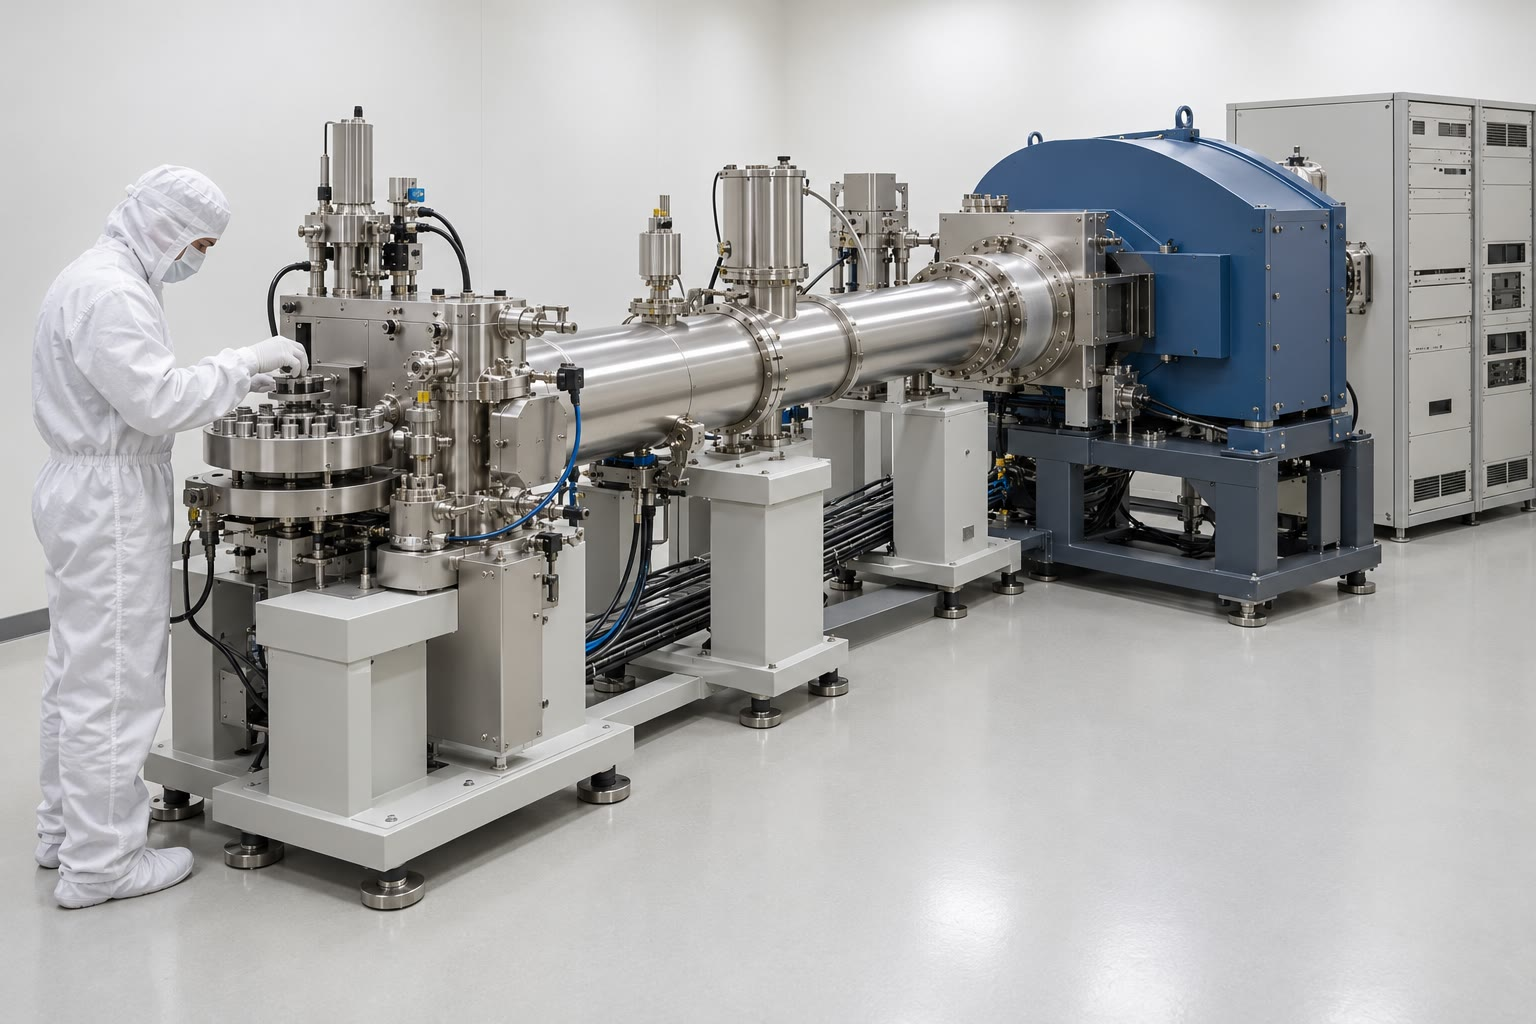
\includegraphics[width=\linewidth]{images/book5/ai/b3-mass-spec-lab.jpg}

{\scriptsize Een massaspectrometer in een schoon laboratorium: de monsterrevolver
links, de vliegbuis en de elektromagneet (Door AI gegenereerde
illustratie.)}
\end{minipage}
\end{inthelab}

\section{Argon--argon-datering}\label{sec:b3:advanced-geochronology:arar}

De kalium--argonmethode uit Boek~3 meet het kalium en
het argon in twee afzonderlijke aliquots van een mineraal. De argon--argonmethode
meet alleen argon, in één aliquot, als isotopenverhoudingen. Het monster wordt
met snelle neutronen bestraald in de kern van een kernreactor, waar de
reactie $^{39}\mathrm{K}(n,p)^{39}\mathrm{Ar}$ een vaste fractie van zijn
kalium-39 omzet in argon-39, een proxy voor kalium. Een mineraal van bekende ouderdom, de
monitor, wordt ernaast bestraald.
% ledger: nmgrl:arar, amherst:arar

\begin{definition}[Argon--argon-datering, J-factor, ouderdomsspectrum, plateau-ouderdom]
\label{def:b3:advanced-geochronology:arar}
\emph{$^{40}\mathrm{Ar}/^{39}\mathrm{Ar}$-datering}\index{argon--argon-datering@$^{40}\mathrm{Ar}/^{39}\mathrm{Ar}$-datering}
dateert een kaliumhoudend mineraal aan de hand van de verhouding $R =
{}^{40}\mathrm{Ar}^*/{}^{39}\mathrm{Ar}_{\mathrm K}$ van zijn radiogene argon-40
tot het argon-39 dat uit zijn kalium door neutronenbestraling is gemaakt. De
\emph{J-factor}\index{J-factor} van een bestraling is $J = (e^{\lambda
t_m} - 1)/R_m$, gevonden uit een monitor van bekende ouderdom $t_m$ en gemeten
verhouding $R_m$, met $\lambda$ de totale vervalconstante van kalium-40. Wanneer het monster
in stappen van toenemende temperatuur wordt ontgast, zet het
\emph{ouderdomsspectrum}\index{ouderdomsspectrum} de ouderdom van elke stap uit tegen de
cumulatieve fractie van vrijgekomen argon-39. Een
\emph{plateau-ouderdom}\index{plateau-ouderdom} is de gewogen gemiddelde ouderdom van opeenvolgende stappen die
binnen hun onzekerheden overeenkomen en een groot deel van het argon-39 vrijmaken.
\end{definition}

\begin{theorem}[De argon--argonouderdom]\label{thm:b3:advanced-geochronology:arar}
Een monster dat met een monitor is bestraald, heeft de ouderdom
\[
t = \frac1\lambda\ln(1 + JR).
\]
\end{theorem}

\begin{proof}
Het radiogene argon is $^{40}\mathrm{Ar}^* = (\lambda_e/\lambda)\,
{}^{40}\mathrm{K}\,(e^{\lambda t} - 1)$, volgens het vertakkend verval uit
Boek~3. Het gevormde argon-39 is $^{39}\mathrm{Ar}_{\mathrm K} =
{}^{39}\mathrm{K}\,\Phi$, waarbij $\Phi$ de neutronendosis en de
werkzame doorsnede van de reactie samenvat. Dus $R = (e^{\lambda t} - 1)/J$ met $J =
\lambda\,\Phi\,{}^{39}\mathrm{K}/(\lambda_e\,{}^{40}\mathrm{K})$. De verhouding
$^{40}\mathrm{K}/^{39}\mathrm{K}$ is in al het kalium gelijk, en $\Phi$ is
gelijk voor twee naast elkaar bestraalde monsters, dus $J$ is gelijk voor het monster
en de monitor; de ouderdom en verhouding van de monitor geven hem, en het omkeren van $R$ geeft
$t$.
\end{proof}

De constanten zijn die van de kalium--argonmethode, $\lambda =
\qty{5.543e-10}{yr^{-1}}$. Een gebruikelijke monitor is een sanidien uit een vulkanische tuf
gedateerd op \qty{28.201}{\Ma}; een monitorverhouding $R_m = 1.3129$ geeft $J =
0.01200$. Atmosferisch argon, met $^{40}\mathrm{Ar}/^{36}\mathrm{Ar} = 295.5$,
wordt afgetrokken met het argon-36 dat in elke stap is gemeten, en argon dat door
neutronen uit calcium en uit kalium zelf is gemaakt, wordt gecorrigeerd met zouten die
in hetzelfde pakket zijn bestraald.
% ledger: schaen20:monitors, amherst:constants, nmgrl:arar

Stapsgewijs verhitten is de kracht van de methode. Het monster wordt in een oven
of met een laser in stappen van toenemende temperatuur verhit, en elke stap levert een
ouderdom op. Als het mineraal sinds het afkoelen gesloten is gebleven, komen alle stappen overeen: het spectrum is
vlak. Als het argon uit de randen van de korrels is verloren, zijn de eerste stappen, die
uit de randen komen, zijn jonger, en de ouderdommen stijgen als een trap naar een
plateau dat door de kernen wordt bepaald. De aanbevolen criteria voor een plateau zijn
ten minste vijf opeenvolgende stappen die meer dan \qty{50}{\percent} van het
argon-39 bevatten, zonder trend tussen hen; de stappen bij lage temperatuur van een trap
worden doorgaans gelezen als verlies van radiogeen argon. Overmaat aan argon, ingesloten uit een
vloeistof toen het mineraal groeide, werkt andersom: het maakt sommige stappen te oud,
meestal de eerste en de laatste, in een zadelvormig spectrum. De som van alle
stappen, de totaalgasouderdom, is wat een kalium--argonouderdom zou hebben opgeleverd: een
gemiddelde dat de geschiedenis verbergt.
% ledger: schaen20:plateau, nmgrl:arar

\begin{omfigure}
\begin{tikzpicture}
\begin{groupplot}[group style={group size=2 by 1, horizontal sep=1.5cm},
  omrecord, height=0.38\linewidth, title style={font=\small},
  xlabel={cumulatief vrijgegeven $^{39}\mathrm{Ar}$ (\unit{\percent})},
  tick label style={font=\scriptsize}, label style={font=\small}]
\nextgroupplot[title={(a) het hele spectrum}, width=0.52\linewidth,
  ylabel={schijnbare ouderdom (\unit{\Ma})}, xmin=0, xmax=100, ymin=130, ymax=320,
  xtick={0,20,40,60,80,100}, ytick={150,200,250,300}]
% computed in figdata/bachelor-3/arar_spectrum.py
\addplot[omDef, thick] table[x=cum, y=age] {figdata/out/bachelor-3-arar_spectrum-boxes.dat};
\node[font=\scriptsize, anchor=west] at (axis cs:12,180) {argonverlies};
\node[font=\scriptsize, anchor=north, red!70!black] at (axis cs:59,290) {plateau};
\nextgroupplot[title={(b) het plateau, vergroot}, width=0.44\linewidth,
  xmin=15, xmax=100, ymin=290, ymax=300, xtick={20,40,60,80,100},
  ytick={290,292,294,296,298,300}]
\addplot[name path=hi, draw=none, forget plot] table[x=cum, y=hi] {figdata/out/bachelor-3-arar_spectrum-boxes.dat};
\addplot[name path=lo, draw=none, forget plot] table[x=cum, y=lo] {figdata/out/bachelor-3-arar_spectrum-boxes.dat};
\addplot[omDef!25, forget plot] fill between[of=hi and lo];
\addplot[omDef, thick] table[x=cum, y=age] {figdata/out/bachelor-3-arar_spectrum-boxes.dat};
\draw[red!70!black, thick] (axis cs:18,296.1) -- (axis cs:100,296.1);
\node[font=\scriptsize, anchor=south, red!70!black] at (axis cs:59,290.3) {plateau-ouderdom \qty[separate-uncertainty=true]{296.1 \pm 0.8}{\Ma}};
\end{groupplot}
\end{tikzpicture}

\par\smallskip{\small Het kunstmatige \omterm{def:b3:advanced-geochronology:arar}{ouderdomsspectrum} van een biotiet uit het graniet van
de eerste figuur: elke stap is getekend op zijn ouderdom, zijn breedte is het aandeel
argon-39 dat hij heeft vrijgegeven. (a) Drie stappen bij lage temperatuur stijgen als een
trap naar een plateau. (b) De zeven plateaustappen, die \qty{82}{\percent} van het
argon-39, met hun bereiken van twee standaardafwijkingen (gearceerd) en de
\omterm{def:b3:advanced-geochronology:arar}{plateau-ouderdom} (rood).}\label{fig:b3:advanced-geochronology:spectrum}
\end{omfigure}

\section{Neodymium-modelouderdommen}\label{sec:b3:advanced-geochronology:model-age}

Wanneer een smelt uit de mantel wordt onttrokken om continentale korst te vormen, blijft samarium,
het meer compatibele element, sterker achter dan neodymium: de nieuwe korst heeft een lagere
$^{147}\mathrm{Sm}/^{144}\mathrm{Nd}$ dan zijn bron, ongeveer 0.13 voor de meeste
korstgesteenten, tegenover 0.1966 voor het chondritische reservoir. Zijn
$^{143}\mathrm{Nd}/^{144}\mathrm{Nd}$ groeit dan trager. Eenmaal gevormd heeft een
korstgesteente de neiging zijn samarium--neodymiumverhouding te behouden, door erosie,
sedimentatie en zelfs omsmelting, zodat zijn neodymium onthoudt wanneer het de
mantel heeft verlaten.
% ledger: white08:model-age, white:chur

\begin{definition}[Modelouderdom]\label{def:b3:advanced-geochronology:model-age}
De \emph{modelouderdom}\index{modelouderdom} van een gesteente in een isotopensysteem is het
tijdstip waarop zijn verhouding, teruggeprojecteerd met zijn huidige moeder--dochterverhouding,
gelijk is aan die van een modelreservoir. Voor neodymium gebruikt $T_{\mathrm{CHUR}}$
het chondritische uniforme reservoir en $T_{\mathrm{DM}}$ de verarmde
mantel.
\end{definition}

\begin{theorem}[Modelouderdom]\label{thm:b3:advanced-geochronology:model-age}
Een monster met huidige verhoudingen $I_s = {}^{143}\mathrm{Nd}/^{144}\mathrm{Nd}$ en
$R_s = {}^{147}\mathrm{Sm}/^{144}\mathrm{Nd}$, vergeleken met een reservoir met huidige
verhoudingen $I_m$ en $R_m$, heeft de \omterm{def:b3:advanced-geochronology:model-age}{modelouderdom}
\[
T = \frac1\lambda\ln\left(1 + \frac{I_s - I_m}{R_s - R_m}\right),
\qquad \lambda = \lambda_{147}.
\]
\end{theorem}

\begin{proof}
Een gesloten systeem had een tijd $T$ geleden de verhouding $I - R(e^{\lambda T} - 1)$:
de isochroonvergelijking, achteruit gelezen. Door dit voor het monster en het
reservoir gelijk te stellen volgt $I_s - I_m = (R_s - R_m)(e^{\lambda T} - 1)$.
\end{proof}

Met $\lambda_{147} = \qty{6.524e-12}{yr^{-1}}$ zijn de reservoirs het chondritische,
vandaag 0.512638 en 0.1966, en het verarmde mantelreservoir,
vandaag 0.51315, ongeveer $\varepsilon_{\mathrm{Nd}} = +10$, wat een gesloten
evolutie vanaf chondritische waarden sinds \qty{4.55}{\Ga} geeft met de verhouding
$^{147}\mathrm{Sm}/^{144}\mathrm{Nd} = 0.2137$. Een verzonnen graniet met
$I_s = 0.511900$ en $R_s = 0.1100$ heeft vandaag $\varepsilon_{\mathrm{Nd}} = -14.4$
$T_{\mathrm{CHUR}} = \qty{1.30}{\Ga}$ en $T_{\mathrm{DM}} =
\qty{1.84}{\Ga}$. De figuur hieronder laat beide zien. De \omterm{def:b3:advanced-geochronology:model-age}{modelouderdom} ten opzichte van de verarmde mantel is de
betere schatting, omdat de korst wordt onttrokken aan een mantel die al
verarmd was; het is de gemiddelde ouderdom waarop het neodymium van het monster de mantel verliet,
zijn korstverblijfsouderdom. Twee voorbehouden beperken hem: de korst mag sindsdien
haar samarium--neodymiumverhouding niet hebben veranderd, en een gesteente dat door het mengen van oude
korst met nieuwe mantelsmelten is ontstaan, heeft een betekenisloze tussenliggende \omterm{def:b3:advanced-geochronology:model-age}{modelouderdom}.
% ledger: villa20:sm147, white:chur, white08:model-age

\begin{omfigure}
\begin{tikzpicture}
\begin{axis}[omrecord, width=0.72\linewidth, height=0.38\linewidth,
  xlabel={tijd voor het heden (\unit{\Ga})}, ylabel={$\varepsilon_{\mathrm{Nd}}$},
  xmin=0, xmax=2.5, ymin=-17, ymax=13, x dir=reverse,
  xtick={0,0.5,1,1.5,2,2.5}, xticklabels={0,0.5,1,1.5,2,2.5},
  tick label style={font=\scriptsize}, label style={font=\small},
  legend style={font=\scriptsize, at={(0.5,1.03)}, anchor=south, legend columns=3, legend cell align=left}]
% computed in figdata/bachelor-3/model_ages.py
\addplot[omDef, thick] table[x=t, y=eps_dm] {figdata/out/bachelor-3-model_ages-evolution.dat};
\addlegendentry{verarmde mantel}
\addplot[black, thick, densely dashed] coordinates {(0,0) (2.5,0)};
\addlegendentry{CHUR}
\addplot[red!70!black, thick] table[x=t, y=eps_sample] {figdata/out/bachelor-3-model_ages-evolution.dat};
\addlegendentry{graniet}
\draw[densely dotted] (axis cs:1.30,0) -- (axis cs:1.30,-17) node[above right, font=\scriptsize, rotate=90] {$T_{\mathrm{CHUR}}$};
\draw[densely dotted] (axis cs:1.84,5.4) -- (axis cs:1.84,-17) node[above right, font=\scriptsize, rotate=90] {$T_{\mathrm{DM}}$};
\end{axis}
\end{tikzpicture}

\par\smallskip{\small $\varepsilon_{\mathrm{Nd}}$ van een verzonnen graniet teruggerekend in de tijd
met zijn eigen samarium--neodymium-verhouding (rood). Het raakt het
chondritisch reservoir bij $T_{\mathrm{CHUR}} = \qty{1.30}{\Ga}$ en de verarmde
mantel (blauw) bij $T_{\mathrm{DM}} = \qty{1.84}{\Ga}$.}\label{fig:b3:advanced-geochronology:model-age}
\end{omfigure}

\section{Splijtingssporen en helium}\label{sec:b3:advanced-geochronology:low-t}

Uranium-238 vervalt ook, zeer zelden, door spontane splijting: de kern
splitst in twee fragmenten die uiteenvliegen en een spoor van schade in de
kristal achterlaten, tot \qty{9}{nm} breed en ongeveer \qty{23}{\micro\metre} lang in
apatiet. Na etsen met zuur worden de sporen zichtbaar onder de microscoop.
Ze herstellen wanneer het kristal wordt verwarmd, bij ongeveer 20 tot \qty{350}{\celsius},
afhankelijk van het mineraal; in apatiet worden ze korter in de gedeeltelijke
uitgloeizone, ongeveer 60 tot \qty{120}{\celsius}, en verdwijnen ze daarboven.
% ledger: kohn24:ft, sueoka19:closure

\begin{definition}[Splijtingssporendatering, uitgloeien van sporen]\label{def:b3:advanced-geochronology:fission-track}
\emph{Splijtingssporendatering}\index{splijtingssporendatering} dateert een mineraal aan de hand van
de dichtheid van de sporen die door spontane splijting van
uranium-238 erin zijn achtergelaten, vergeleken met het uraniumgehalte. \emph{Uitgloeien
van sporen}\index{uitgloeien van sporen} is het korter worden en verdwijnen van de
sporen door herstel van het kristal wanneer het wordt verwarmd.
\end{definition}

\begin{theorem}[De splijtingssporenouderdom]\label{thm:b3:advanced-geochronology:fission-track}
Met $\lambda_f$ de vervalconstante van spontane splijting en $\lambda =
\lambda_{238}$ de totale, heeft een kristal met $N_s$ spontane splijtingen per
volume-eenheid en $N$ atomen uranium-238 de ouderdom
\[
t = \frac1\lambda\ln\left(1 + \frac{\lambda}{\lambda_f}\,\frac{N_s}{N}\right).
\]
In het laboratorium wordt het uranium gemeten door splijting van
uranium-235 op te wekken met thermische neutronen, en wordt de ouderdom
\[
t = \frac1\lambda\ln\left(1 + \lambda\,\zeta\,g\,\rho_d\,\frac{\rho_s}{\rho_i}\right),
\]
met $\rho_s$ en $\rho_i$ de dichtheden van de spontane en de geïnduceerde sporen,
$\rho_d$ de sporendichtheid van een dosimeterglas, $g = 0.5$ een geometriefactor
en $\zeta$ een kalibratieconstante die op standaarden van bekende ouderdom is bepaald.
\end{theorem}

\begin{proof}
Uranium-238 is $N(e^{\lambda t} - 1)$ keer vervallen, en de fractie
$\lambda_f/\lambda$ van deze vervallen waren splijtingen: $N_s =
(\lambda_f/\lambda)N(e^{\lambda t} - 1)$, wat omgewerkt de eerste vorm geeft.
De sporendichtheden zijn evenredig met $N_s$ en met het aantal geïnduceerde
splijtingen, $N\,\sigma\,\Phi/137.8$, waarin $\sigma$ de splijtingsdoorsnede
van uranium-235 is en $\Phi$ de neutronenfluentie, zelf evenredig met
$\rho_d$. De verhouding $\rho_s/\rho_i$ is dan $N_s/N$ maal een product van
constanten, en $\lambda_f$, $\sigma$, $137.8$ en het rendement van het etsen en
tellen worden samen met $g$ in $\zeta$ ondergebracht.
\end{proof}

De vervalconstante voor splijting is slechts bekend tot binnen ongeveer \qty{10}{\percent},
tussen \num{7.9e-17} en \qty{8.7e-17}{yr^{-1}}, en daarom geven de meeste
laboratoria de voorkeur aan de $\zeta$-kalibratie. De lengte van de sporen bewaart
een spoor van het temperatuurverloop. Een gesteente dat snel door de
gedeeltelijke uitgloeizone afkoelde, heeft lange sporen van vrijwel gelijke
lengte; een gesteente dat er lang in verbleef, heeft kortere sporen met sterk
uiteenlopende lengten, en dan is de splijtingssporenouderdom een gemengde
ouderdom, geen tijdstip van een passage door één temperatuur.
% ledger: kohn24:ft

\begin{omfigure}
\begin{tikzpicture}[scale=0.85]
% (a) an etched apatite grain with tracks
\draw[thick, fill=omLithLime!15] (0,0) -- (3.2,0) -- (3.8,1.0) -- (3.2,2.0) -- (0,2.0) -- (-0.6,1.0) -- cycle;
\foreach \x/\y/\a in {0.4/0.5/30, 1.2/1.3/-20, 2.0/0.6/75, 2.6/1.4/10, 0.9/1.6/110, 1.7/0.9/150, 2.9/0.8/50}
  {\draw[very thick, black] (\x,\y) -- ++(\a:0.45);}
\node[font=\small] at (1.6,-0.4) {(a) geëtste sporen in apatiet};
% (b) alpha ejection from a grain
\begin{scope}[xshift=6cm]
\draw[thick, fill=omLithLime!15] (0,0) rectangle (3.4,2.0);
\draw[dashed] (0.35,0.35) rectangle (3.05,1.65);
\fill[black] (0.2,1.0) circle (1.5pt) node[below right, font=\scriptsize] {U};
\draw[->, red!70!black, thick] (0.2,1.0) -- ++(160:0.7) node[left, font=\scriptsize] {He verloren};
\fill[black] (1.7,1.0) circle (1.5pt);
\draw[->, red!70!black, thick] (1.7,1.0) -- ++(40:0.5);
\node[font=\scriptsize, align=center] at (1.7,0.55) {He behouden};
\draw[<->] (3.05,1.8) -- (3.4,1.8) node[right, font=\scriptsize] {\qty{20}{\micro\metre}};
\node[font=\small] at (1.7,-0.4) {(b) alfa-uitstoot};
\end{scope}
\end{tikzpicture}

\par\smallskip{\small Schematisch. (a) Spontane splijtingssporen, zichtbaar gemaakt door
etsen op een gepolijste apatietkorrel, worden per oppervlakte-eenheid geteld. (b) Een alfadeeltje
legt ongeveer \qty{20}{\micro\metre} af: deeltjes die binnen die
afstand van het oppervlak zijn uitgezonden (buiten de gestippelde lijn), kunnen de korrel verlaten, zodat een
kleine korrel minder van zijn helium behoudt.}\label{fig:b3:advanced-geochronology:low-t}
\end{omfigure}
% ledger: zeigler23:ejection

Elk alfaverval zendt een heliumkern-4 uit. Uranium, thorium en hun ketens
hopen helium op in een kristal, dat het alleen vasthoudt wanneer het koel is.

\begin{definition}[(U--Th)/He-datering, zone van gedeeltelijke retentie]\label{def:b3:advanced-geochronology:uthhe}
\emph{(U--Th)/He-datering}\index{U--Th/He-datering@(U--Th)/He-datering} dateert een
mineraal aan de hand van het door alfavervalen van uranium, thorium
en hun dochters opgehoopte helium-4, vergeleken met zijn uranium- en thoriumgehalte. De \emph{zone van gedeeltelijke
retentie}\index{zone van gedeeltelijke retentie} is het temperatuurbereik waarin
het geproduceerde helium gedeeltelijk wordt behouden en gedeeltelijk door diffusie verloren gaat.
\end{definition}

\begin{theorem}[Heliumgroei]\label{thm:b3:advanced-geochronology:helium}
Een kristal dat gedurende een tijd $t$ voor helium gesloten is, bevat
\[
\mathrm{He} = 8\,{}^{238}\mathrm U\,(e^{\lambda_{238}t} - 1)
+ 7\,{}^{235}\mathrm U\,(e^{\lambda_{235}t} - 1)
+ 6\,{}^{232}\mathrm{Th}\,(e^{\lambda_{232}t} - 1),
\]
in atomen, met de ouders vandaag gemeten; samarium-147 voegt een kleine term toe.
\end{theorem}

\begin{proof}
Elke keten verliest zijn massaverschil in alfadeeltjes, telkens vier massa-eenheden:
$(238 - 206)/4 = 8$, $(235 - 207)/4 = 7$, $(232 - 208)/4 = 6$, terwijl
bètavervalingen het massagetal niet veranderen. Elke keten verkeert in secular evenwicht,
dus elk verval van een moeder wordt gevolgd door de hele keten, en het aantal
vervallen van elke moeder is gelijk aan dat in de ouderdomsvergelijking.
\end{proof}

Voor een jong kristal geldt $e^{\lambda t} - 1 \approx \lambda t$, en de ouderdom volgt
uit een enkele deling. Een alfadeeltje legt ongeveer
\qty{20}{\micro\metre} af voordat het tot stilstand komt, verliest een kristal dus het helium dat
dicht bij het oppervlak is gevormd; de gemeten ouderdom wordt gedeeld door de behouden fractie $F_T$,
die kleiner is voor kleine korrels ($F_T = 0.70$ betekent dat \qty{30}{\percent}
verloren gaat). Apatiet sluit voor helium bij ongeveer 50 tot \qty{80}{\celsius}, zirkoon bij
160 tot \qty{200}{\celsius}: met apatietsplijtingssporen, bij ongeveer 90 tot
\qty{120}{\celsius} dateren de laagtemperatuurchronometers de laatste paar
kilometers van de opstijging van een gesteente naar het oppervlak, zoals ze
in \cref{ch:b3:orogenic-wedges} zijn gebruikt.
% ledger: zeigler23:ejection, sueoka19:closure, iaea:isotopes

\section{Kosmogene nuclides}\label{sec:b3:advanced-geochronology:cosmogenic}

Kosmische straling die de atmosfeer treft, vormt deeltjesbuien van secundaire deeltjes. De
snelle neutronen die de grond bereiken, breken kernen in de mineralen van de bovenste
meters gesteente, door spallatie: zuurstof in kwarts wordt beryllium-10, silicium
wordt aluminium-26. Muonen maken sommige nuclides dieper en domineren onder ongeveer
\qty{3}{m}.
% ledger: zech04:exposure, portenga:method

\begin{definition}[Kosmogeen nuclide, blootstellingsouderdom, productiesnelheid]
\label{def:b3:advanced-geochronology:cosmogenic}
Een \emph{kosmogeen nuclide}\index{kosmogeen nuclide} is een nuclide dat in
een mineraal aan of nabij het oppervlak wordt gevormd door de secundaire deeltjes van kosmische straling. Zijn
\emph{productiesnelheid}\index{productiesnelheid (kosmogeen)} $P$ is het aantal
atomen die per eenheid van massa mineraal en per jaar worden gevormd. De
\emph{blootstellingsouderdom}\index{blootstellingsouderdom} van een oppervlak is de tijd sinds het voor het eerst aan
kosmische straling werd blootgesteld, bepaald uit de concentratie van een kosmogeen nuclide.
\end{definition}

De \omterm{def:b3:advanced-geochronology:cosmogenic}{productiesnelheid} neemt af met de diepte als $P_0e^{-\rho z/\Lambda}$, waarbij
de verzwakkingslengte wordt gesteld op $\Lambda = \qty{160}{g.cm^{-2}}$, ongeveer
\qty{60}{cm} graniet met een dichtheid van \qty{2.7}{g.cm^{-3}}. Aan het oppervlak
neemt de waarde toe met de hoogte, omdat minder lucht de rots afschermt, en met
de geomagnetische breedte, omdat het veld minder deeltjes afbuigt nabij de
polen. Productiesnelheden worden gegeven voor een referentie op zeeniveau en hoge breedte en
worden geschaald naar elke locatie: één kalibratie levert $P_0 = \num{4.96}\text{ atomen}\,\unit{g^{-1}.yr^{-1}}$
van beryllium-10 in kwarts bij die referentie. Beryllium-10 heeft een halveringstijd van
\qty{1.388}{Myr}, $\lambda = \qty{4.994e-7}{yr^{-1}}$.
% ledger: balco08:params, zech04:exposure, lugaro:slr-table

\begin{theorem}[Blootstelling met verval en erosie]\label{thm:b3:advanced-geochronology:exposure}
Een oppervlak dat met een constante snelheid $\varepsilon$ wordt verlaagd en gedurende een tijd $t$ blootgesteld,
zonder overgeërfd nuclide, heeft aan zijn oppervlak de concentratie
\[
N(t) = \frac{P_0}{\mu}\bigl(1 - e^{-\mu t}\bigr), \qquad
\mu = \lambda + \frac{\rho\varepsilon}{\Lambda}.
\]
Zonder erosie geldt $N = (P_0/\lambda)(1 - e^{-\lambda t})$; na lange tijd
$N = P_0/\mu$, en zonder verval is dit de formule $P_0\Lambda/(\rho\varepsilon)$
die in Boek~3 staat.
\end{theorem}

\begin{proof}
Volg de korrel die vandaag aan het oppervlak ligt. Een tijd $s$ geleden lag zij op de
diepte $\varepsilon s$, waar zij atomen won met de snelheid $P_0e^{-\rho\varepsilon
s/\Lambda}$; van die atomen is de fractie $e^{-\lambda s}$ vandaag nog over. Door
te sommeren over de blootstelling,
\[
N = \int_0^t P_0e^{-\rho\varepsilon s/\Lambda}e^{-\lambda s}\,\mathrm ds
= \frac{P_0}{\mu}\bigl(1 - e^{-\mu t}\bigr).
\]
De grenzen volgen door $\varepsilon = 0$ te nemen, $t \to \infty$ te laten gaan, en
dan $\lambda = 0$.
\end{proof}

Zonder erosie verzadigt de concentratie op $P_0/\lambda$ na een paar
halveringstijden: een oppervlak bereikt \qty{90}{\percent} daarvan na $\ln 10/\lambda
= \qty{4.6}{Myr}$, en daarna is er geen datering meer mogelijk. Met erosie,
wordt de stationaire toestand sneller bereikt, na enkele keren $1/\mu$, en de
concentratie levert $\varepsilon$; de snelheid wordt gemiddeld over de tijd
$\Lambda/(\rho\varepsilon)$ die de korrel nodig had om door één
verzwakkingslengte te stijgen, enkele tienduizenden jaren bij snelheden van enkele
tientallen meters per miljoen jaar. Ontsluitingen van vaste gesteente eroderen met
enkele meters tot enkele tientallen meters per miljoen jaar; stroomgebieden, gemeten aan het
zand van hun rivieren, sneller.
% ledger: portenga:rates, portenga:method

Twee nucliden met verschillende halveringstijden dateren begraving. Beryllium-10 en
aluminium-26 worden samen gevormd in kwarts in een vaste verhouding; wanneer een korrel
diep in een grot of onder dik sediment begraven is, stopt de productie, en
aluminium-26, dat sneller vervalt, blijft achter: de verhouding van de twee
neemt met de tijd af en dateert de begraving.

\section{De statistiek van een ouderdom}\label{sec:b3:advanced-geochronology:statistics}

Een ouderdom komt met zijn onzekerheid, en een reeks ouderdommen met de vraag
of ze met elkaar overeenkomen. Laat $n$ metingen $x_i$ van één grootheid
met standaardafwijkingen $\sigma_i$ hebben. Hun gewogen gemiddelde is $\bar x = \sum w_ix_i/W$, met
$w_i = 1/\sigma_i^2$ en $W = \sum w_i$, en de standaardafwijking daarvan is
$1/\sqrt W$.

\begin{definition}[Gemiddeld kwadraat van de gewogen afwijkingen]\label{def:b3:advanced-geochronology:mswd}
Het \emph{gemiddeld kwadraat van de gewogen afwijkingen}\index{gemiddeld kwadraat van de gewogen afwijkingen}
(MSWD) van $n$ metingen rond een gefit model met $p$ aangepaste parameters
is
\[
\mathrm{MSWD} = \frac{1}{n - p}\sum_i \frac{(x_i - \hat x_i)^2}{\sigma_i^2},
\]
waarbij $\hat x_i$ de modelwaarde is: $p = 1$ voor een gewogen gemiddelde, $p = 2$ voor
een rechte lijn, zoals een isochroon of een \omterm{def:b3:advanced-geochronology:concordia}{discordia}.
\end{definition}

\begin{proposition}[De MSWD heeft verwachtingswaarde één]\label{prop:b3:advanced-geochronology:mswd}
Als de $x_i$ onafhankelijk en normaal verdeeld zijn, met gemiddelde $\mu$ en de
standaardafwijkingen $\sigma_i$, dan heeft de MSWD rond hun gewogen gemiddelde verwachtingswaarde 1.
\end{proposition}

\begin{proof}
We splitsen $x_i - \mu = (x_i - \bar x) + (\bar x - \mu)$ op en gebruiken $\sum
w_i(x_i - \bar x) = 0$,
\[
\sum w_i(x_i - \mu)^2 = \sum w_i(x_i - \bar x)^2 + W(\bar x - \mu)^2.
\]
Links heeft elke term verwachtingswaarde 1, dus heeft de som verwachtingswaarde $n$. Rechts
heeft $\bar x$ variantie $1/W$, dus heeft de laatste term verwachtingswaarde 1.
Daaruit volgt dat $\sum w_i(x_i - \bar x)^2$ verwachtingswaarde $n - 1$ heeft.
\end{proof}

De MSWD spreidt zich des te meer rond 1 naarmate er minder vrijheidsgraden zijn,
$f = n - p$: de bovengrens bij \qty{95}{\percent} is ongeveer $1 +
2\sqrt{2/f}$, 2.63 voor $f = 3$ en 2.15 voor $f = 6$. Boven die grens
spreiden de metingen zich meer dan hun onzekerheden toelaten: de monsters
hebben niet allemaal dezelfde ouderdom, of het systeem is verstoord. Ver onder 1
zijn de onzekerheden overschat.
% ledger: schaen20:mswd

\begin{method}[Een isochroon fitten met fouten op beide assen]\label{met:b3:advanced-geochronology:york}
Wanneer beide coördinaten fouten $\sigma_{x,i}$, $\sigma_{y,i}$ dragen, gecorreleerd
met de coëfficiënt $r_i$, zoals bij uranium--lood- en isochroondata:
\begin{enumerate}
\item begin met de helling $b$ van de gewone kleinste-kwadratenlijn;
\item geef elk punt het gewicht $W_i = 1/(\sigma_{y,i}^2 + b^2\sigma_{x,i}^2 -
2br_i\sigma_{x,i}\sigma_{y,i})$, de inverse variantie van de afstand tot de
lijn, gemeten langs $y$;
\item fit de gewogen lijn met deze gewichten, wat een nieuwe $b$ oplevert, en
keer terug naar stap 2 totdat $b$ niet meer verandert;
\item bereken de MSWD met de gewichten $W_i$ en $n - 2$ vrijheidsgraden,
en de onzekerheid van de helling en het snijpunt uit de laatste gewichten.
\end{enumerate}
Met $\sigma_{x,i} = 0$ hangen de gewichten niet van $b$ af, en de methode
gaat over in de gewogen kleinste kwadraten van $y$ op $x$ zoals die in de oefeningen wordt gebruikt.
\end{method}

De onzekerheid van een vervalconstante is voor elke ouderdom van één systeem dezelfde:
ze speelt geen rol wanneer ouderdommen van één systeem worden vergeleken, maar moet
worden opgeteld wanneer ouderdommen uit twee systemen worden vergeleken. De vervalconstante van samarium-147 is bijvoorbeeld
bekend tot op ongeveer \qty{0.4}{\percent}; die van kalium-40,
dat vertakkend en traag vervalt, beperkt de nauwkeurigheid van argonouderdommen.
% ledger: villa20:sm147, nmgrl:arar


\section{Oefeningen}

\begin{exercise}[$\star$]\label{exo:b3:advanced-geochronology:1}
Een zirkoon heeft $^{206}\mathrm{Pb}^*/^{238}\mathrm{U} = 0.04500$ en
$^{207}\mathrm{Pb}^*/^{235}\mathrm{U} = 0.3300$. Bereken zijn twee
uranium--lood-ouderdommen. Is hij concordant? Aan welke kant van de \omterm{def:b3:advanced-geochronology:concordia}{concordia}
ligt hij?
\end{exercise}
% ledger: amherst:constants

\begin{exercise}[$\star$]\label{exo:b3:advanced-geochronology:2}
Een monitor van \qty{28.201}{\Ma} geeft $R_m = 1.3129$. Bereken $J$ met $\lambda
= \qty{5.543e-10}{yr^{-1}}$, en daarna de ouderdom van een monster van dezelfde bestraling
met $R = 10.000$ (gebruik $J = 0.01200$).
\end{exercise}
% ledger: schaen20:monitors

\begin{exercise}[$\star$]\label{exo:b3:advanced-geochronology:3}
Een schalie heeft $^{143}\mathrm{Nd}/^{144}\mathrm{Nd} = 0.51180$ en
$^{147}\mathrm{Sm}/^{144}\mathrm{Nd} = 0.1200$. Bereken zijn $T_{\mathrm{CHUR}}$
en $T_{\mathrm{DM}}$ met de waarden uit het hoofdstuk.
\end{exercise}
% ledger: villa20:sm147, white:chur, white08:model-age

\begin{exercise}[$\star$]\label{exo:b3:advanced-geochronology:4}
Een zwerfkei van kwarts op een morene op de referentielocatie bevat \num{2.0e5}
atomen beryllium-10 per gram. Neem aan dat er geen erosie en geen overerving is,
bereken de \omterm{def:b3:advanced-geochronology:cosmogenic}{blootstellingsouderdom} eerst zonder en daarna met verval, met $P_0 =
\num{4.96}\text{ atomen}\,\unit{g^{-1}.yr^{-1}}$.
\end{exercise}
% ledger: balco08:params, lugaro:slr-table

\begin{exercise}[$\star\star$]\label{exo:b3:advanced-geochronology:5}
Toon aan dat de \omterm{def:b3:advanced-geochronology:concordia}{concordia} nabij de oorsprong een lijn is met helling
$\lambda_{238}/\lambda_{235}$, en bereken die helling. Verklaar waarom de \omterm{def:b3:advanced-geochronology:concordia}{discordia} van
kristallen die pas zeer recent lood hebben verloren door de oorsprong gaat, en
wat de lood--lood-ouderdom van zulke kristallen meet.
\end{exercise}

\begin{exercise}[$\star\star$]\label{exo:b3:advanced-geochronology:6}
Vier stapouderdommen van een plateau zijn $296.4 \pm 0.8$, $295.1 \pm 1.0$, $297.0 \pm
0.9$ en \qty[separate-uncertainty=true]{295.8 \pm 0.7}{\Ma} ($1\sigma$). Bereken hun gewogen gemiddelde,
hun standaardafwijking en de MSWD. Komen ze overeen?
\end{exercise}
% ledger: schaen20:mswd

\begin{exercise}[$\star\star$]\label{exo:b3:advanced-geochronology:7}
Een apatiet heeft $\rho_s = \qty{1.20e6}{cm^{-2}}$ en $\rho_i =
\qty{2.40e6}{cm^{-2}}$, met $\rho_d = \qty{1.10e6}{cm^{-2}}$, $g = 0.5$ en een
laboratoriumkalibratie $\zeta = \qty{350}{yr.cm^2}$. Bereken zijn
splijtingssporenouderdom. Welke gebeurtenis dateert hij?
\end{exercise}
% ledger: kohn24:ft, sueoka19:closure

\begin{exercise}[$\star\star$]\label{exo:b3:advanced-geochronology:8}
Een apatiet bevat \qty{20}{ppm} uranium (\qty{99.2742}{\percent}
uranium-238, \qty{0.7204}{\percent} uranium-235 naar atomen), \qty{40}{ppm}
thorium-232 (halveringstijd \qty{1.40e10}{yr}) en \qty{1.0}{nmol.g^{-1}} helium.
Bereken zijn (U--Th)/He-ouderdom met de lineaire benadering, en daarna de
ouderdom gecorrigeerd voor alfa-uitstoot met $F_T = 0.75$.
\end{exercise}
% ledger: iaea:isotopes, zeigler23:ejection

\begin{exercise}[$\star\star$]\label{exo:b3:advanced-geochronology:9}
Bereken voor beryllium-10 op de referentielocatie de verzadigingsconcentratie
zonder erosie en de tijd om \qty{90}{\percent} daarvan te bereiken. Bereken de
stationaire concentratie van een oppervlak dat erodeert met \qty{10}{m.Myr^{-1}} (graniet,
\qty{2.7}{g.cm^{-3}}, $\Lambda = \qty{160}{g.cm^{-2}}$).
\end{exercise}
% ledger: balco08:params, zech04:exposure, lugaro:slr-table

\begin{exercise}[$\star\star\star$]\label{exo:b3:advanced-geochronology:10}
Twee metingen $x_1 \pm \sigma_1$ en $x_2 \pm \sigma_2$ van één ouderdom worden
gecombineerd. Toon aan dat hun MSWD ten opzichte van het gewogen gemiddelde gelijk is aan
$(x_1 - x_2)^2/(\sigma_1^2 + \sigma_2^2)$, en bewijs rechtstreeks dat de
verwachtingswaarde 1 is wanneer beide dezelfde ouderdom meten.
\end{exercise}

\begin{exercise}[$\star\star\star$]\label{exo:b3:advanced-geochronology:11}
Een zirkoon van \qty{2700}{\Ma} verloor lood bij \qty{500}{\Ma} en heeft vandaag
$^{206}\mathrm{Pb}^*/^{238}\mathrm{U} = 0.300$. Welk deel van zijn lood verloor hij?
Bereken zijn $^{207}\mathrm{Pb}^*/^{235}\mathrm{U}$, zijn twee uranium--lood-ouderdommen
en, door iteratie, zijn lood--lood-ouderdom. Welke van de drie ouderdommen heeft
een betekenis?
\end{exercise}

\begin{exercise}[$\star\star\star$]\label{exo:b3:advanced-geochronology:12}
Een oppervlak van vaste gesteente op de referentielocatie bevat \num{1.0e6} atomen van
beryllium-10 per gram. Bereken de \omterm{def:b3:advanced-geochronology:cosmogenic}{blootstellingsouderdom} bij aanname van geen erosie, en
vervolgens de erosiesnelheid bij aanname van een stationaire toestand. Toon aan dat elk paar $(t, \varepsilon)$
tussen deze twee grenzen bij de meting past, en zeg welke tweede
meting ze zou kunnen scheiden.
\end{exercise}

\section{Probleem: Zirkonen van de Varden-graniet}

\begin{problem}[{Weekendprobleem --- de kristallisatie, afkoeling en
blootlegging van een verzonnen graniet, gelezen aan vier klokken}]\label{pb:b3:advanced-geochronology:1}
Het graniet van de Varden Hills, de verzonnen regio van de reeks, werd tegen het Trias
blootgelegd, vervolgens begraven onder de mesozoïsche bedekking en weer naar het
oppervlak gebracht. Vijf van zijn zirkonen geven, met een-standaarddeviatiefouten op $y$
(neem $x$ als exact):
\begin{center}
\small
\begin{tabular}{|l|ccccc|}
\hline
zirkoon & Z1 & Z2 & Z3 & Z4 & Z5 \\
\hline
$x = {}^{207}\mathrm{Pb}^*/^{235}\mathrm U$ & 0.3467 & 0.3260 & 0.3027 & 0.2793 & 0.2535 \\
$y = {}^{206}\mathrm{Pb}^*/^{238}\mathrm U$ & 0.04794 & 0.04505 & 0.04207 & 0.03892 & 0.03553 \\
$\sigma_y$ & 0.00010 & 0.00009 & 0.00008 & 0.00008 & 0.00007 \\
\hline
\end{tabular}
\end{center}
Gebruik de constanten van het hoofdstuk. Alle analyses zijn oefengegevens.
% ledger: amherst:constants, schaen20:monitors, schaen20:plateau, schaen20:mswd, sueoka19:closure, balco08:params, lugaro:slr-table

\medskip\noindent\textbf{Deel I --- De zirkonen.}
\begin{enumerate}
\item Bereken de twee uranium--lood-ouderdommen van elke zirkoon. Zijn ze concordant?
\item Waarom nemen de ouderdommen af van Z1 tot Z5, met $t_{207} > t_{206}$
voor elk?
\item Bereken de Tera--Wasserburg-coördinaten van Z1 en Z5.
\item Bereken met de gewichten $w_i = 1/\sigma_{y,i}^2$ de gewogen gemiddelden
$\bar x$ en $\bar y$ en $S_{xx} = \sum w_i(x_i - \bar x)^2$.
\item Bereken de helling $b = \sum w_i(x_i - \bar x)(y_i - \bar y)/S_{xx}$ en
het snijpunt $a$ van de \omterm{def:b3:advanced-geochronology:concordia}{discordia}.
\item Vergelijk $b$ met de helling van de \omterm{def:b3:advanced-geochronology:concordia}{concordia} nabij \qty{310}{\Ma}. Wat
voorspelt dit?
\end{enumerate}

\medskip\noindent\textbf{Deel II --- De snijpunten.}
\begin{enumerate}[resume]
\item Zoek het \omterm{def:b3:advanced-geochronology:concordia}{bovenste snijpunt} met de methode van Newton, startend bij \qty{310}{\Ma}.
\item Zoek het \omterm{def:b3:advanced-geochronology:concordia}{onderste snijpunt}, startend bij \qty{100}{\Ma}.
\item Bereken de gewogen residuen en de MSWD. Is de fit aanvaardbaar?
\item De standaarddeviatie van de helling is $1/\sqrt{S_{xx}}$. Bereken haar.
\item Draai de lijn om $(\bar x, \bar y)$ naar de hellingen $b \pm 2s_b$ en
herbereken het \omterm{def:b3:advanced-geochronology:concordia}{bovenste snijpunt} voor elk. Wat is de onzekerheid van de ouderdom?
\item Welk deel van zijn lood verloor Z1, en Z5?
\end{enumerate}

\medskip\noindent\textbf{Deel III --- De biotiet.} Een biotiet van het graniet,
bestraald met een monitor van \qty{28.201}{\Ma} die $R_m = 1.3129$ oplevert, wordt
in tien stappen ontgast:
\begin{center}
\small
\setlength{\tabcolsep}{5pt}\begin{tabular}{|l|cccccccccc|}
\hline
stap & 1 & 2 & 3 & 4 & 5 & 6 & 7 & 8 & 9 & 10 \\
$^{39}\mathrm{Ar}$ (\unit{\percent}) & 4 & 6 & 8 & 12 & 14 & 15 & 14 & 12 & 9 & 6 \\
$R$ & 7.225 & 11.226 & 13.937 & 14.891 & 14.820 & 14.869 & 14.918 & 14.847 & 14.907 & 14.804 \\
ouderdom (\unit{\Ma}) & & 228.0 & 279.0 & & 295.3 & 296.2 & 297.1 & 295.8 & 296.9 & \\
$\sigma$ (\unit{\Ma}) & 0.6 & 0.9 & 1.0 & 1.1 & 1.1 & 1.1 & 1.1 & 1.1 & 1.1 & 1.1 \\
\hline
\end{tabular}
\end{center}
\begin{enumerate}[resume]
\item Bereken $J$; rond af op 0.01200.
\item Bereken de ouderdommen van de stappen 1, 4 en 10.
\item Welke stappen vormen een plateau volgens de criteria van het hoofdstuk?
\item Bereken de \omterm{def:b3:advanced-geochronology:arar}{plateau-ouderdom}, de standaarddeviatie ervan en de MSWD.
\item Bereken de totale-gasverhouding en -ouderdom. Waarom is die jonger dan het plateau?
\item Ga ervan uit dat het graniet bij \qty{700}{\celsius} kristalliseerde en de
biotiet bij \qty{375}{\celsius} sluit, en bereken de gemiddelde afkoelingssnelheid.
\item Wat kan er bij het \omterm{def:b3:advanced-geochronology:concordia}{onderste snijpunt} zijn gebeurd?
Is het argonspectrum daarmee in overeenstemming?
\end{enumerate}

\medskip\noindent\textbf{Deel IV --- De blootlegging.} Vier apatieten, bemonsterd op
een helling van de heuvels, geven (U--Th)/He-ouderdommen van 43.1, 46.0, 49.2 en
\qty{52.0}{\Ma} bij 310, 370, 430 en \qty{490}{m}. De top van het graniet,
op een flauwe heuvelkam op een locatie waar $P_0 = \num{5.6}\text{ atomen}\,\unit{g^{-1}.yr^{-1}}$,
bevat \num{1.64e5} atomen beryllium-10 per gram kwarts.
\begin{enumerate}[resume]
\item Bereken de helling van de \omterm{def:b3:orogenic-wedges:age-elevation}{ouderdom--hoogterelatie}, in meter per miljoen jaar.
million years.
\item Bij een sluitingstemperatuur van \qty{65}{\celsius}, een oppervlaktetemperatuur van
\qty{10}{\celsius} en een geoterm van \qty{30}{\celsius.km^{-1}} op welke diepte
de laagste apatiet sloot. Welke gemiddelde blootleggingssnelheid volgt sindsdien?
\item Bereken de huidige erosiesnelheid uit het beryllium-10, bij aanname van een
stationaire toestand.
\item Welke snelheid geeft de formule uit Boek~3, zonder verval?
\item Over welke tijd wordt de beryllium-10-snelheid gemiddeld? Vergelijk de
drie snelheden.
\item Geef de kristallisatieouderdom van het Varden-graniet met zijn
onzekerheid.
\end{enumerate}
\end{problem}
